\begin{figure}[htbp]
	\centering
	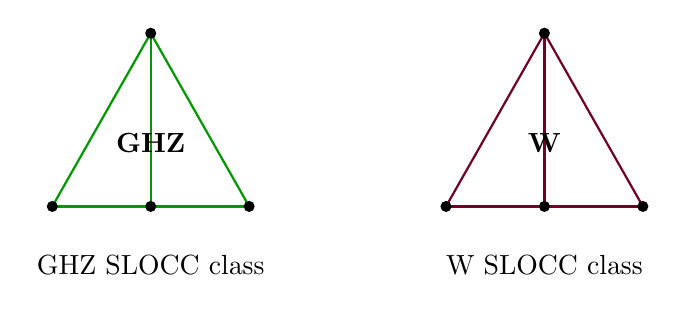
\begin{tikzpicture}[scale=1.0]
		\draw[thick, green!60!black] (0,0) -- (2.5,0) -- (1.25,2.2) -- cycle;
		\draw[thick, green!60!black] (1.25,0) -- (1.25,2.2);
		\draw[thick, green!60!black] (0,0) -- (1.25,0);
		\draw[thick, green!60!black] (2.5,0) -- (1.25,0);
		\foreach \p in {(0,0), (2.5,0), (1.25,2.2), (1.25,0)}
		\fill[black] \p circle (2pt);
		\node at (1.25,0.8) {\textbf{GHZ}};

		\draw[thick, purple!60!black, xshift=5cm] (0,0) -- (2.5,0) -- (1.25,2.2) -- cycle;
		\draw[thick, purple!60!black, xshift=5cm] (1.25,0) -- (1.25,2.2);
		\draw[thick, purple!60!black, xshift=5cm] (0,0) -- (1.25,0);
		\draw[thick, purple!60!black, xshift=5cm] (2.5,0) -- (1.25,0);
		\foreach \p in {(5,0), (7.5,0), (6.25,2.2), (6.25,0)}
		\fill[black] \p circle (2pt);
		\node at (6.25,0.8) {\textbf{W}};

		\node[below] at (1.25,-0.5) {GHZ SLOCC class};
		\node[below] at (6.25,-0.5) {W SLOCC class};

	\end{tikzpicture}
	\caption{Three-qubit entanglement polytope showing the two SLOCC equivalence classes (GHZ and W) as separate tetrahedra. Each tetrahedron has 4 vertices corresponding to product states; states in different classes cannot be converted into each other by SLOCC operations.}
	\label{fig:entanglement-polytope-3qubit}
\end{figure}
